% Nallino, Part I p. 193: Schiaparelli's figure for the declination of a star, redrawn from the print: the sphere as
% an arc of a circle from the lower end of the ecliptic over the top to Y; the equator OY and the ecliptic OX as
% straight lines; the arcs QST and PSV; OQ, OP and TZ (the arc QST produced) in dashes, each where it printed; the
% bold italic letters and the italic words aequator and ecliptica. Measured on the scan (_intake/latin/tools/fig193).
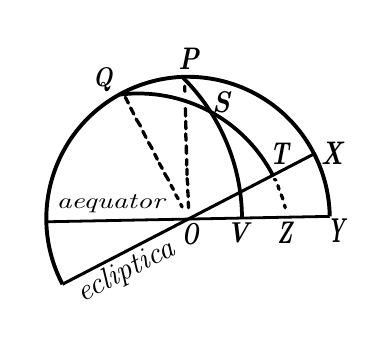
\begin{tikzpicture}[x=0.9928pt,y=-0.9928pt,line cap=butt,every node/.style={font=\fontsize{11}{11}\bfseries\itshape\selectfont,inner sep=0pt}]
\useasboundingbox (0,0) rectangle (120.00,104.00);
\draw[line width=1.01pt] (6.81,70.65) -- (109.94,68.68);  % the equator
\draw[line width=1.10pt] (12.67,93.37) -- (104.27,45.93);  % the ecliptic
\draw[line width=1.41pt] (12.67,93.37) arc[start angle=152.38,end angle=359.14,radius=51.58];
\draw[line width=1.35pt] (33.29,24.39) arc[start angle=-97.24,end angle=-27.45,radius=55.21];
\draw[line width=1.36pt] (56.26,17.93) arc[start angle=-45.54,end angle=-0.37,radius=72.63];
% the dashes of OQ, OP and TZ
\draw[line width=1.19pt,line cap=round] (35.53,25.35)--(36.66,27.47) (37.46,29.19)--(38.64,31.46) (39.47,33.24)--(41.09,35.85) (41.90,37.71)--(43.08,39.98) (43.97,41.77)--(45.34,44.09) (46.23,46.00)--(47.19,47.91) (47.88,49.32)--(49.00,51.27) (49.81,53.01)--(51.31,55.56);
\draw[line width=1.19pt,line cap=round] (52.15,57.32)--(53.05,58.91) (53.86,60.80)--(54.80,62.30) (55.70,64.23)--(56.23,65.27) (57.13,21.32)--(57.21,23.17) (57.40,29.39)--(57.49,32.20) (57.53,34.10)--(57.59,36.80) (57.50,38.64)--(57.66,41.01) (57.75,42.99)--(57.77,45.79);
\draw[line width=1.19pt,line cap=round] (57.89,47.96)--(57.84,50.05) (58.01,51.44)--(57.96,53.53) (58.02,54.92)--(58.28,57.18) (58.23,59.14)--(58.44,61.49) (58.46,63.45)--(58.52,65.54) (89.79,55.19)--(90.33,55.45) (91.08,57.47)--(91.48,58.84) (92.30,60.81)--(92.88,62.36);
\draw[line width=1.19pt,line cap=round] (93.50,64.59)--(93.74,65.52);
\node at (58.54,11.51) {\normalfont\fontsize{11}{11}\bfseries\itshape\selectfont \resizebox{7.38pt}{7.73pt}{P}};
\node at (27.32,18.97) {\normalfont\fontsize{11}{11}\bfseries\itshape\selectfont \resizebox{7.11pt}{6.70pt}{Q}};
\node at (70.42,26.99) {\normalfont\fontsize{11}{11}\bfseries\itshape\selectfont \resizebox{6.46pt}{7.39pt}{S}};
\node at (91.58,45.93) {\normalfont\fontsize{11}{11}\bfseries\itshape\selectfont \resizebox{6.87pt}{7.85pt}{T}};
\node at (110.76,45.77) {\normalfont\fontsize{11}{11}\bfseries\itshape\selectfont \resizebox{7.98pt}{8.09pt}{X}};
\node at (59.22,75.21) {\normalfont\fontsize{11}{11}\bfseries\itshape\selectfont \resizebox{6.21pt}{7.49pt}{O}};
\node at (76.48,74.77) {\normalfont\fontsize{11}{11}\bfseries\itshape\selectfont \resizebox{8.02pt}{7.13pt}{V}};
\node at (93.60,74.77) {\normalfont\fontsize{11}{11}\bfseries\itshape\selectfont \resizebox{5.51pt}{7.74pt}{Z}};
\node at (112.29,73.73) {\normalfont\fontsize{11}{11}\bfseries\itshape\selectfont \resizebox{6.32pt}{8.56pt}{Y}};
\node at (30.12,63.95) {\normalfont\fontsize{11}{11}\itshape\selectfont \resizebox{39.02pt}{4.94pt}{aequator}};
\node[rotate=27.38] at (35.72,88.75) {\normalfont\fontsize{11}{11}\itshape\selectfont \resizebox{38.10pt}{7.58pt}{ecliptica}};
\end{tikzpicture}
